
\subsection{Hybrid SRP-PHAT}

Peterson \cite{peterson2005hybrid} describes a novel approach for sound localization using a two stage approach in order to reduce the computational load. The first stage roughly identifies the sources locations while the second stage is a modified version of the SRP-PHAT algorithm that only performs a grid search around the estimated location from the first stage.  The method is well suited for near-field localization using large aperture array which is not our requirement but the idea can be adapted in the case of far-field sound localization. Section \ref{sec:TDOA} gives an introduction to TDOA based localization and introduces the cone approximation for the far-field. The idea of the hybrid approach is to do a classical GCC-PHAT estimation to get the relative delays between the sensors. The delays estimates are used to derive the cone intersections which give a location estimate which is then input into a SRP-PHAT algorithm where the search region is constrained around the location estimates. A system overview of the algorithm is given in figure \ref{fig:hybridalgo}.

\begin{figure}[H]
    \centering
    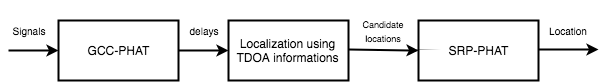
\includegraphics[width=1\textwidth]{Figures/hybridalgo.png}
    \caption{Simplified block diagram of the Hybrid algorithm}
    \label{fig:hybridalgo}
\end{figure}

\subsection{Improvements on SRP}

In \cite{salvati2017exploiting} the author proposes a method to improve the computational efficiency and coherence of the grid search using discreet sampling information where the method is called geometrically sampled grid (GSG). \cite{do2007real} uses Stochastic Region Contraction(SRC) to reduce the computational time of the search. \cite{salvati2014incoherent} introduces an incoherent Frequency Fusion based on a normalized arithmetic mean (NAM) which improves the localization performance of SRP, MVDR and MUSIC. Salvati \cite{salvati2015frequency} introduces a SRP weighted MVDR, which combines machine learning power to the noise resilience of the MVDR beamformer, the method is improved in \cite{salvati2016use} by using SVM training. SRP-WMVDR is proved to be much more resilient to noise and better than SRP-PHAT for SNR up to 0. All of those papers used a microphone array composed of more than 8 microphones. Few experimental data are available for the case of 4 microphones and none for the case of a tetrahedral array, whereby a ULA is mostly used for the different test methods.


